%%%%%%%%%%%%%%%%%%%%%%%%%%%%%%%%%%%%%%%%%%%%
\subsection{Work-flow overview}

The ultimate goal of the PFS validation \& commissioning work-flow is to optimize the PFS performance and validate the goodness for scientific use.
To achieve this goal, we proceed the PFS commissioning following this outline:
\begin{enumerate}
\item Integrate PFS subsystems of which the performances have been validated by the PFS collaborators.
\item Operate the system and confirm their functions on the telescope.
\item Characterize the system, e.g. by calibrating the coordinate systems to put the fibers on the targets with required accuracy.
\item Evaluate the on-sky performance and validate it. \\
Firstly we focus on verifying the performances at given telescope positions, rotation angles even if we cannot confirm the same performance at all positions.
\item Finally, stabilize the instrument performances. \\
We optimize software, re-configuration sequence, calibration and so on.
We validate the performance at any telescope pointing or time.
\end{enumerate}

The latest top-level requirements are described on the following page: \\
{\tt http://sumire.pbworks.com/w/page/76118150/System\%20level\%20requirements}\\
See also the compliance matrix in section \ref{sec:cmatrix}.

\bigskip

The work-flow of the PFS commissioning (Fig. \ref{fig:flowchart}) consists of five parts: 
\begin{enumerate}
\item Validation of MCS (labeled with M-\#, see section \ref{sec:MCS})
 \begin{itemize}
 \item Validation of MCS basic functions.
 \item Pre-study of the coordinate transformation using pinhole array or FMOS/PIR or pinhole array on POpt2.
 \end{itemize}
This part requires only MCS.
\item Validation of PFI (labeled with P-\#, see section \ref{sec:PFI}), basically prior to SpS delivery at Subaru.
 \begin{itemize}
 \item Alignment of WFC with the primary mirror.
 \item Telescope pointing analysis.
 \item AG camera validation.
 \item Confirmation of PFI--MCS relation (registration of Fixed Fiducial Fibers in F3C).
 \item Make the first-pass distortion map using AGCs (sky).
 \end{itemize}
This part requires only PFI basically, but some sequences need MCS, too.
\item Validation of SpS (labeled with S-\#, see section \ref{sec:SpS})
 \begin{itemize}
 \item Validation of image quality and stability in the SCR.
 \item Characterization of SMs.
 \end{itemize}
This part requires SMs and SCR.
We don't need the telescope to carry out this part.
\item Validation of FoCCoS--Cable B (labeled with F-\#, see section \ref{sec:FoCCoS})
 \begin{itemize}
 \item Validation of cable connection.
 \item Confirmation of fibers ID on MCS and SpS.
 \end{itemize}
This part requires all subsystems: MCS, PFI, Cable B and SpS.
\item Commissioning all systems (labeled with A-\#, see section \ref{sec:All}
 \begin{itemize}
 \item Cobra calibration.
 \item PSF characterization.
 \item Make the second-pass distortion map using fibers (sky).
 \item Validation of all observational sequence.
 \item Performance verification.
 \item Stabilization of the instrument performance and operation.
 \end{itemize}
This part requires all subsystems: MCS, PFI, Cable B and SpS.
\end{enumerate}

During the commissioning procedure, we also verify the software sequence for observation (acquisition, fiber configuration, guiding, and exposure) at suitable commissioning sequences.
We also verify the data reduction pipeline (DRP).

%---------------------------------------------------
% Figure: Big picture of the PFS commissioning
%---------------------------------------------------
\begin{landscape}
\begin{figure}[!ht]
\begin{center}
\vspace*{-10mm}
\hspace*{-5mm}
\includegraphics[width=255mm]{PFScommissioning.pdf}
\end{center}
\vspace*{-8mm}
\caption{Flowchart of Validation \& Commissioning. Larger one is available on the PBworks: \newline
http://sumire.pbworks.com/w/file/101350174/PFScommissioning.pdf
%http://member.ipmu.jp/yuki.moritani/tmp/PFS/PFScommissioning.pdf
}
\label{fig:flowchart}
\end{figure}
\end{landscape}

%%% Subsystem I \& T and capable functions at delivery
\subsection{Subsystem I \& T (TBD)}
\subsubsection{I \& T at Subaru}
Each subsystem is delivered to Subaru separately.
After the delivery, collaborators will re-assemble modules (if needed) and test their performance.
In this section, the brief summary of I\&T of subsystems are described.
See the documents by collaborators (TBA) for detailed procedure of I\&T.

Table \ref{tbl:SubSysIandT} summarizes schedule and place of I\&T of subsystems.
The validated functions before shipping (or before commissioning) is listed in table \ref{tbl:subfuncs}.

%---------------------------------------------------
% Table: Subsystem functions at delivery.
%---------------------------------------------------
\begin{table}[!ht]
\begin{center}
\caption{Subsystem I\&T time and place.}
%\scriptsize
%\footnotesize
\begin{tabular}{*{3}{c}}\label{tbl:SubSysIandT} \\ \hline
Subsystem	& Year/Month & I\&T Place \\ \hline \hline
PFI	& 2019/04--2019/05		& TBD \\
MCS	& 2017/03--2017/06	& Observation floor \\
SpS-SM1,2	& 2017/07--08		& IR4 (SCR) \\
SpS-SM3,4	& 2018/05--06		& IR4 (SCR) \\
Cable B	&	2018/12--2019/02	& TBD \\ \hline
\end{tabular} 
\end{center}
\end{table}

\paragraph{PFI}
PFI is shipped after assembled at ASIAA, so it doesn't need to be re-assembled at Subaru.
%, according to the latest I\&T story board.
%After shipped, PFI is re-adjusted if needed.
The I\&T story board at the summit is in preparation but the currently assumed test items are as follows:
\begin{enumerate}
\item Fiber transparency tests
\item Rotational test for Cable Wrapper
\item Power on/off test (fiducial fiber illuminator etc.)
\item Image acquisition (central camera, fiducial fiber viewing cameras, and AG cameras)
\item Cobra circular motion test
\item Dot position check
\item Cobra convergence test with dummy MCS
\item AG camera test for dark and noise
\end{enumerate}
These test are carried out using test stand on which PFI will be shipped, and dummy MCS.
Because the tilt mechanism is not assumed to be delivered so far, the test should be limited compared to AIT phase at ASIAA.

After the above tests are passed, PFI will be installed to POpt2, and the the same tests are repeated, except for the cobra circular motion test.

\redtext{Test items for software --- control individual modules, telemetry, communicate with MLP1/STS etc.}

\paragraph{MCS}
After AIT at ASIAA, MCS camera modules are disassemble for shipping to Subaru. 
The camera modules, therefore, will be re-assembled in Hawaii.
After it, the image quality will be checked with the pinhole array.
If the test will be done firstly at Hilo base, re-assemble and test should be also carried out at the summit.
ASIAA is planning optional configuration to adjust the alignment of MCS with respect to the prime focus, because MCS will be mounted to CsBox only ``mechanically".
If the pinhole array can be equipped on Popt2, MCS can be aligned with the prime focus by checking the camera image.
Such a test enables us to use time efficiently before PFI arrival, and to save time after PFI arrival, which is expected one year later than MCS arrival, because we should align MCS with the prime focus firstly.


\redtext{Test items for software --- control individual modules, telemetry, communicate with STS etc.}

\paragraph{SpS}
After AIT at LAM, four modules are shipped to Subaru two by two.
The modules are re-assembled in SCR on the IR4 floor, and the following test will be carried out (TBC):
\begin{itemize}
\item Thermal function (cooling down /warming up)
\item Image quality
\item Characterization of spectrograph  (optional: TBD)
\end{itemize}

\redtext{Test items for software --- control individual modules, telemetry, communicate with STS etc.}

\paragraph{Cable B}
After shipped to Subaru, the light-path will be tested firstly. 
It is still to be discussed, but we will also execute FRD measurement with simple equipment for some fibers as aliveness test.
Then the cable is installed to the telescope, while the fiber connection monitoring system is installed to the IR3 floor.
It is desirable to measure FRD on the telescope, but details are to be discussed.
The details is TBC.

\redtext{Test items for software?}

\subsubsection{Complementarity between subsystem I\& T and the commissioning}
To be written.



%---------------------------------------------------
% Table: Subsystem functions at delivery.
%---------------------------------------------------
%%%%%%%%%%%%%%%%%%%%%%%%%%%%%%%%%%%%%%%%%%%%
%%% Table of Compliance Matrix


%--------------------------------------------------------------
%  Table: expected runs and nights
%--------------------------------------------------------------
%\setlength{\tabcolsep}{1mm}{
\begin{landscape}
\begin{longtable}{r|p{100mm}|p{25mm}|c|p{30mm}|p{50mm}}
%\begin{center}
\caption{
The list of validated functions before the commissioning.}
\label{tbl:subfuncs} 
%\scriptsize
\footnotesize
\\ \hline
No	& Functions & No. of Table \ref{tbl:funcs} & Succ.?  & Req.	& Notes \\ \hline \hline
\endhead
%\hline
\endfoot
%%% PFI
\multicolumn{6}{l}{\hspace{5mm} {\bf PFI (including Cable C)}} \\ \hline
%%% Initial check
P01	& Instrument rotator moves from $-278 \degree$ to $+278 \degree$.	& 8	&	&	& \\ \hline
P02	& Positioning error of A\&C camera is $\sim$ 2.8 um.	& 25	&	&	& CDR \\ \hline
P03 & PFI has 97 fiducial fibers.	&	& 	& {\tt REQ-FOC-L3-267}	& CDR \\ \hline 
P04 & All fiducial fibers can be back-illuminated.	&  28, 30	& 	& {\tt REQ-L3-PFI-008}	& \\ \hline
P05 & Science fibers home position is measured in the accuracy of 50 um PTV.	& 34, 35	& 	&	& Relative position to a fiducial fiber near the center. \\ \hline
P06 & Science fibers rotation center is measured in the accuracy of 50 um PTV.	& 34, 35	& 	&	& Relative position to a fiducial fiber near the center. \\ \hline
P07 & Perimeter fiducial fibers position is measured in the accuracy of 50 um PTV.	& 34, 26	& 	&	& Relative position to a fiducial fiber near the center. \\ \hline
P08 & Field element dots position is measured in the accuracy of 50 um PTV.	& 34, 35	& 	&	& Relative position to a fiducial fiber near the center. \\ \hline
P09 & The position of AG camera fiducial fibers is measured in the accuracy of 10 um PTV.	& 26	& 	&	& Relative to nearest perimeter fiducial fiber. \\ \hline
P10 & The position of AG camera sensors is measured in the accuracy of 10 um PTV.	& 	& 	&	& Relative to nearest perimeter fiducial fiber. \\ \hline
P11 & The focus position of science fibers is measured in the accuracy of 12 um PTV.	& 	& 	&	& Relative to designed focus position. \\ \hline
P12 & The focus position of perimeter fiducial fibers is measured in the accuracy of 12 um PTV.	& 	& 	&	& Relative to designed focus position. \\ \hline
P13 & The focus position of AG camera sensors is measured in the accuracy of 12 um PTV.	& 	& 	&	& Relative to designed focus position. \\ \hline
P14 & The tilt of science fibers is measured in the accuracy of $0.17 \degree$ PTV.	& 	& 	&	& Relative to a fiducial fiber near the center. \\ \hline
P15 & The tilt of perimeter fiducial fibers is measured in the accuracy of $0.17 \degree$ PTV.	& 	& 	&	& Relative to a fiducial fiber near the center. \\ \hline
P16 & The tilt of AG camera sensors is measured in the accuracy of $0.17 \degree$ PTV.	& 	& 	&	& Relative to a COB rear surface. \\ \hline
P17 & P05--P16 are achieved with rotation angle of $0, \pm 60 \degree$ and El. $90,60,30 \degree $	& 	& 	&	& CDR \\ \hline
P18 & The cobra positioner converge to requested x/y position in the accuracy of 10 um PTV.	& 34, 35	& 	&	&  \\ \hline
P19 & P19 is achieved with rotation angle of $0, \pm 60 \degree$ and El. $90,60,30 \degree $	& 	& 	&	& CDR \\ \hline
P21	& AG camera shall acquire image.	& 	& 	& 	& 	\\ \hline
P21	& Fiducial fiber viewing cameras shall acquire image.	& 6	& 	& 	& 	\\ \hline
P22	& Center camera shall acquire image.	& 7	& 	& 	& 	\\ \hline
P21	& PFI shall be operated remotely via MHS.	& 4, 10	& 	& 	& 	\\ \hline
...	& ...	& ...	& ...	& ...	\\ \hline
%%% MCS
\hline
\multicolumn{6}{l}{\hspace{5mm} {\bf MCS}} \\ \hline
M01	& The FoV is large enough to see all science and fiducial fibers at a time.	& 16, 17	&	& {\tt REQ-MET-2} 	& MCS covers 462mm in diameter at the focal plane (CDR).	\\ \hline
M02	& The fiber centroid cam be measured within the error of 5 um (RMS) for all fibers.	& 15, 16, 17, 26	& 	& {\tt REQ-MET-6}	& $<$ 4.46um RMS (CDR)	\\ \hline
M03	& MCS completes one cycle of image acquisition, data read, and measurement within 5 seconds in average. 	& 18 	& 	& {\tt REQ-MET-7}	& $<$ 3 seconds (CDR) 	\\ \hline
M04	& MCS shall be operated remotely via MHS.	& 1,3	& 	& 	& 	\\ \hline
...	& ...	& ...	& ...	& ...	& ...	\\ \hline
%%% SpS
\hline
\multicolumn{6}{l}{\hspace{5mm} {\bf SpS (including Cable A)}} \\ \hline
S01	& The blue detector shall be cooled down to operating temperature ($173 \pm 0.5$ K)	& 	& 	& {\tt SPS-REQ-307}, {\tt SPS-REQ-202}, {\tt SPS-REQ-95}	& 	\\ \hline
S02	& The red detector shall be cooled down to operating temperature ($173 \pm 0.5$ K)	& 	& 	& {\tt SPS-REQ-307}, {\tt SPS-REQ-203}, {\tt SPS-REQ-95}	& 	\\ \hline
S03	& The nir detector shall be cooled down to operating temperature ($110 \pm 0.5$ K)	& 	& 	& {\tt SPS-REQ-307}, {\tt SPS-REQ-204}, {\tt SPS-REQ-95}	& 	\\ \hline
S04	 & All camera units cover 2394 science fibers in their readable area.	& 	& 	& 	& 	\\ \hline
S05	 & SpS shall back-illuminate science fibers.	& 29, 30 	& 	& 	& 	\\ \hline
...	& ...	& ...	& ...	& ...	& ...	\\ \hline
%%% SpS
\hline
\multicolumn{6}{l}{\hspace{5mm} {\bf Cable B}} \\ \hline
F01		& Cable shall deliver 2394 light source from PFI to SpS.	& 14	& 	& {\tt REQ-FOC-L3-267}	& 	\\ \hline
F02		& Cable connection should be monitored remotely. 	& 14	& 	& {\tt REQ-FOC-L3-043}	& 	\\ \hline
...	& ...	& ...	& ...	& ...	& ...	\\ \hline
%...	& ...	& ...	& ...	& ...	& ... \\ \hline \hline
%\end{center}
\end{longtable}
\end{landscape}



%%% achieved functions
\subsection{Achieved PFS Functions during the Commissioning (TBD)}\label{sec:cmatrix}
Table \ref{tbl:funcs} shows achieved PFS functions and related commissioning sequences (compliance matrix).
Column 1 lists the priority of the functions (TBD).

%---------------------------------------------------
% Table: Achieved functions and related sequences.
%---------------------------------------------------
%\begin{table}[!ht]
%\caption{Achieved functions during the commissioning.}
%\label{tbl:funcs}
%\begin{center}
%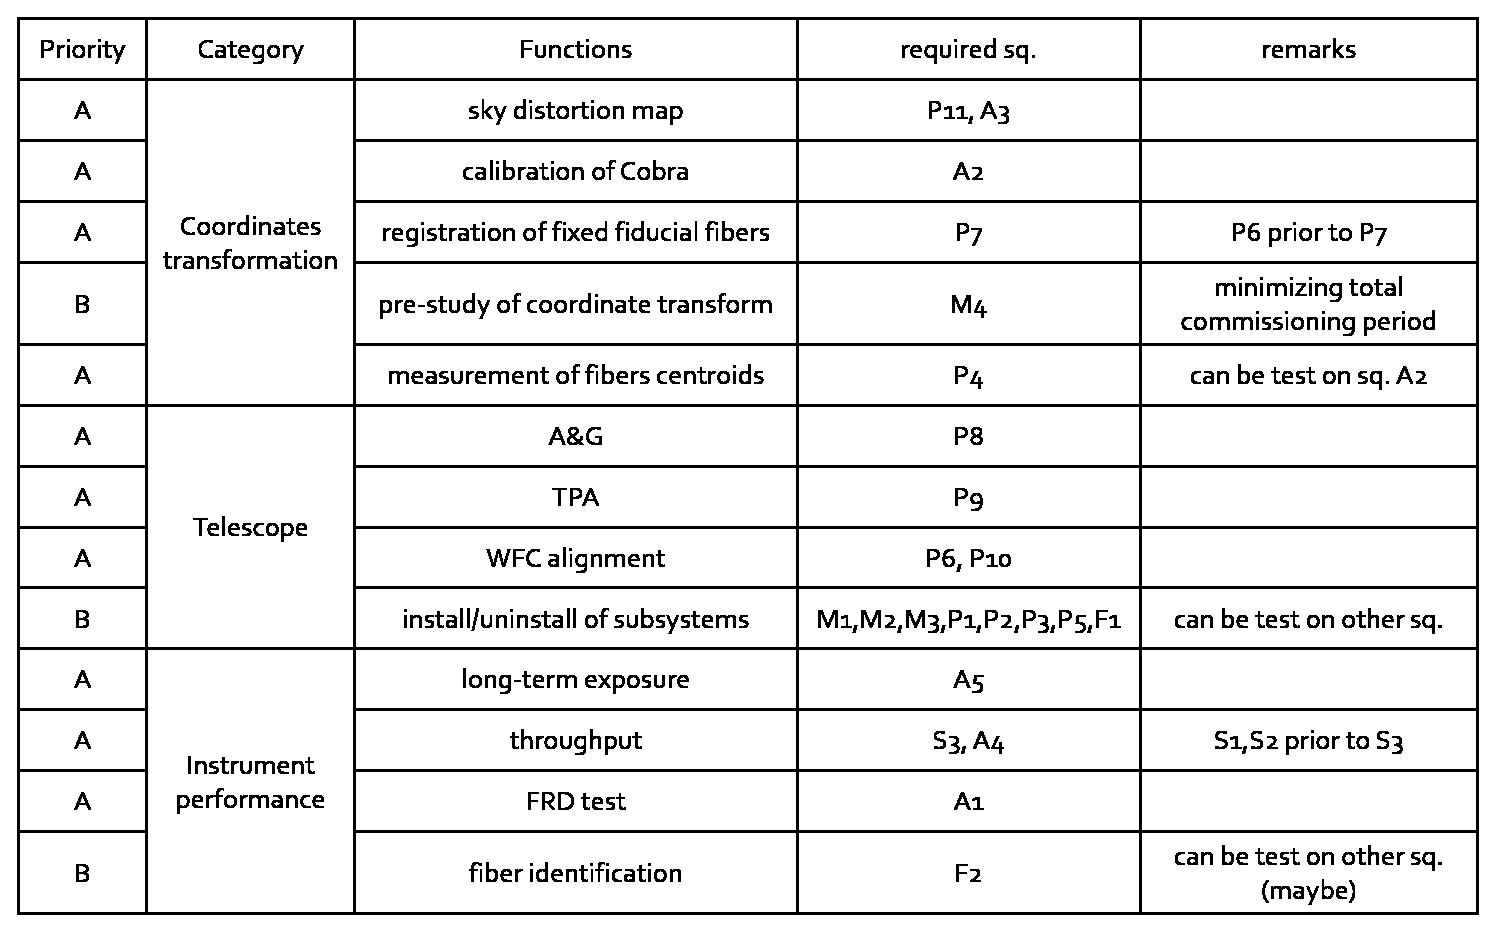
\includegraphics[width=150mm]{AchievedFunctions.eps}
%\end{center}
%\end{table}
%%%%%%%%%%%%%%%%%%%%%%%%%%%%%%%%%%%%%%%%%%%%
%%% Table of Compliance Matrix


%--------------------------------------------------------------
%  Table: expected runs and nights
%--------------------------------------------------------------
%\setlength{\tabcolsep}{1mm}{
\begin{landscape}
\begin{longtable}{r|c|p{50mm}|p{100mm}|p{11mm}|c|p{35mm}}
%\begin{center}
\caption{
The list of achieved functions during the commissioning.}
\label{tbl:funcs} 
%\scriptsize
\footnotesize
\\ \hline
No	& Pri.	& Functions & Success Criteria & \#Sq.  & Succ.?  & Notes \\ \hline \hline
\endhead
%\hline
\endfoot
%%% Fiber allocation
\multicolumn{7}{l}{\hspace{5mm} {\bf Fiber Allocation}} \\ \hline
%%% Initial check
1	& A 	& Initial check of subsystems	& MCS can communicate with MHS	& \ref{secflow:MCSoff}, \ref{secflow:MCSon}	&	& 	\\ \cline{1-2}\cline{4-7}
2	& A 	&	& MCS can take image with required performance (dark, noise,etc.)	& \ref{secflow:MCSoff}, \ref{secflow:MCSon}	&	& 	\\ \cline{1-2}\cline{4-7}
3	& A 	& 	& All mechanical and environmental sensors of MCS can be read	& \ref{secflow:MCSoff}, \ref{secflow:MCSon}	&	&	\\ \cline{1-2}\cline{4-7}
4	& A	&	& PFI can communicate with MHS	& \ref{secflow:PFIoff}, \ref{secflow:PFIon}	&	& \\ \cline{1-2}\cline{4-7}
5	& A	&	& AG cameras can take image with required performance (noise, dark, etc.)	& \ref{secflow:PFIoff}, \ref{secflow:PFIon}	&	& \\ \cline{1-2}\cline{4-7}
6	& A	&	& Fixed fiducial cameras can take image with required performance (noise, dark, etc.)	& \ref{secflow:PFIoff}, \ref{secflow:PFIon}	&	& \\ \cline{1-2}\cline{4-7}
7	& A	&	& Center camera can take image with required performance (noise, dark, etc.)	& \ref{secflow:PFIoff}, \ref{secflow:PFIon}	&	& \\ \cline{1-2}\cline{4-7}
8	& A	&	& Instrument rotator moves from $-270 \degree$ to $+270 \degree$	& \ref{secflow:PFIoff}, \ref{secflow:PFIon}	&	& \\ \cline{1-2}\cline{4-7}
9	& A	&	& Cooling system works	& \ref{secflow:PFIoff}, \ref{secflow:PFIon}	&	& \\ \cline{1-2}\cline{4-7}
10	& A 	& 	& All mechanical and environmental sensors of PFI can be read	& \ref{secflow:PFIoff}, \ref{secflow:PFIon}	&	&	\\ \hline
%%% Installation of subsystems
11	& A 	& Installation of subsystems	& MCS is installed on the Cs focus meeting required accuracy (tilt $<$ 0.14 degree, decenter of optical axis $<$ 45mm in x,y each)	& \ref{secflow:MCSinstall}	&	&	\\ \cline{1-2}\cline{4-7}
12	& A	&	& PFI is installed in POpt2 meeting required repeatability ($<$ 200um in lateral, $<$ 100um in focus, $<$ 15 arcsec in tilt)	& \ref{secflow:PFIoff}, \ref{secflow:PFIoffset}	&	& repeatability of focus and tilt is not measured in \ref{secflow:PFIoffset}  \\ \cline{1-2}\cline{4-7}
13	& A	&	& POpt2 is installed on the prime focus with accuracy of 10 um	& \ref{secflow:PFIinstall}	&	& Specification of Mitsubishi \\ \cline{1-2}\cline{4-7}
14	& A	&	& Cable B is connected with PFI and SpS correctly (fiber ID, throughput?)	& \ref{secflow:FibConcec}, \ref{secflow:FibID}	&	& \\ \hline 
%%% pre study of coordinate transformation
15	& A 	& Pre-study of coordinate transformation	& Algorithm of coordinate transformation works (accuracy: 50 um)	& \ref{secflow:prestudy}	&	&	\\ \hline
%%% measurement of fiber centroids
16	& A	& Measurement of fibers centroids	& Spot size is $\sim$2.6 pix on entire FoV at various Elevations and rotator angles	& \ref{secflow:MCSperf}	&	&	\\ \cline{1-2}\cline{4-7}
17	& A	& 	& Centroids can be measured within the accuracy of 5 um	 (1.5 pixel)	& \ref{secflow:MCSperf}	&	&	\\ \cline{1-2}\cline{4-7}
18	& A	& 	& Measurement process is done within 5 seconds	& \ref{secflow:MCSperf}	&	&	\\ \hline
%%% Telescope pointing and tracking
19	& A	& Telescope pointing and tracing	& Telescope can be focused with error of 10 um	& \ref{secflow:WFCTiltShift}	&	&	\\ \cline{1-2}\cline{4-7}
21	& A	& 	& WFC is aligned to Primary Mirror within the shift of 0.5mm and tilt of 1 arcmin	& \ref{secflow:WFCTiltShift}	&	&	\\ \cline{1-2}\cline{4-7}
23	& A	& 	& Telescope Pointing Analysis can be done with error of XXX	& \ref{secflow:TPA1}	&	&	\\ \cline{1-2}\cline{4-7}
24	& A	& 	& PFS can acquire field and start auto guiding within 15 seconds	& \ref{secflow:AGCfunc}	&	& \\ \cline{1-2}\cline{4-7}
25	& A	& 	& Telescope can track a field with error of $\lesssim$ 0.1 arcsec in both RA and DEC directions using A\&G camera	& \ref{secflow:AGCfunc}	&	& 	\\ \hline
%%% Registration of FFF
26	& A	& Registration of fixed fiducial fibers	& Positions of the fixed fiducial fibers measured on F3C within the accuracy of 5 um (TBD)	& \ref{secflow:mcs2f3c}	& 	& \ref{secflow:WFCTiltShift} is needed prior to \ref{secflow:mcs2f3c}	\\ \hline
%%% First-pass distortion map
27	& A	&	First-pass sky-PFI distortion map	& Fiber allocation error is $<$50 um	& \ref{secflow:1stDM}	&	&	\\ \hline
%%% back illumination of fibers
28	& A	& Back illumination of fibers	& Fixed fiducial fibers are back-illuminated	& \ref{secflow:PFIoff}	&	&	\\ \cline{1-2}\cline{4-7}
29	& A	& 	& Science fibers are back-illuminated	& \ref{secflow:CobraCal}	&	&	\\ \cline{1-2}\cline{4-7}
30	& A	& 	& Brightness of science and fixed fiducial fibers is the same on MCS	& \ref{secflow:CobraCal}	&	&	\\ \hline
%%% Cobra movement/calibration
31	& A	&	Cobra initial movement	& Cobra can move anyhow & \ref{secflow:PFIon}	&	&	\\ \hline
32	& A	&	Calibration of Cobra	& Cobra parameters are calibrated	& \ref{secflow:CobraCal}	&	& \\ \hline
33	& A	&	Cobra movement	& Cobra can move everywhere in their patrol area & \ref{secflow:CobraCal}	&	&	\\ \hline
%%% Second-pass distortion map
34	& A	&	Second-pass sky-PFI distortion map	& Fiber allocation error is $<\sim$10 um (TBD)	& \ref{secflow:raster}	&	&	\\ \hline
%%% Fiber reconfiguration
35	& A	& Fiber configuration	& 95\% of 2394 fibers can be allocated to their targeted position within 105 seconds	& \ref{secflow:PV1}	&	& \\ \hline 
36	& A	& Fiber re-configuration	& Fibers are reconfigured within 105 seconds with the accuracy of 10um (TBD)		& \ref{secflow:PV2}	&	& \\ \hline \hline
%---------------------------
\multicolumn{7}{l}{\hspace{5mm}{\bf Spectrograph}} \\ \hline
%%% Initial check
37	& A	& Initial check of subsystems & SCR and SpS can communicate with MHS	& \ref{secflow:SCR}	&	& \\ \cline{1-2}\cline{4-7}
38	& A	&	& The temperature of SCR is controlled stably (3--5 degC)	& \ref{secflow:SCR}	&	& \\ \cline{1-2}\cline{4-7}
39	& A	&	& SCR ans SpS Can recover from power failure mode	& \ref{secflow:SCR}	&	& \\ \cline{1-2}\cline{4-7}
40	& A	&	& All 12 detectors can take images within expected noise.	& \ref{secflow:SCR}	&	& \\ \cline{1-2}\cline{4-7}
41	& A	&	& SpS can change LR/MR mode in RED arms	& \ref{secflow:SCR}	&	& \\  \cline{1-2}\cline{4-7}
42	& A	&	& SpS can open/close shutters	& \ref{secflow:SCR}	&	& \\  \cline{1-2}\cline{4-7}
43	& A 	& 	& All mechanical and environmental sensors of SMs can be read	& \ref{secflow:SCR}	&	&	\\ \cline{1-2}\cline{4-7}
44	& A	&	& The input light can be focused on the detectors (EE is 50\% in 3 x 3 pixels and 90 \% in 5 x 5 pixels in 90\% of detector area)	& \ref{secflow:SCR}	&	& \\  \hline
%%% Installing subsystems
%A	& Installation of subsystems & \\
%%% Characterization
45	& A	& Characterization	& Wavelength coverage is 380--650 nm in BLUE arms	& \ref{secflow:SpSchar}	&	& \\ \cline{1-2}\cline{4-7}
46	& A	& 	& Wavelength coverage is 630--970 nm in RED(LR) arms	& \ref{secflow:SpSchar}	&	& \\ \cline{1-2}\cline{4-7}
47	& A	& 	& Wavelength coverage is 710--885 nm in RED(MR) arms	& \ref{secflow:SpSchar}	&	& \\ \cline{1-2}\cline{4-7}
48	& A	& 	& Wavelength coverage is 940--1260 nm in NIR arms	& \ref{secflow:SpSchar}	&	& \\ \cline{1-2}\cline{4-7}
49	& A	&	& Spectral resolution is $>$2300 at 520 nm (BLUE)	& \ref{secflow:SpSchar}	&	& \\ \cline{1-2}\cline{4-7}
50	& A	&	& Spectral resolution is $>$2800 at 810 nm (RED, LR)	& \ref{secflow:SpSchar}	&	& \\ \cline{1-2}\cline{4-7}
51	& A	&	& Spectral resolution is $>$5000 at 810 nm (RED, MR)	& \ref{secflow:SpSchar}	&	& \\ \cline{1-2}\cline{4-7}
52	& A	&	& Spectral resolution is $>$4100 at 1100 nm (NIR)	& \ref{secflow:SpSchar}	&	& \\ \cline{1-2}\cline{4-7}
53	& A	&	& Throughput of SpS (TBD)	& \ref{secflow:SpSchar}	&	& \\ \cline{1-2}\cline{4-7}
54	& A	&	& PSF and spectral distribution of SpS are characterized	& \ref{secflow:SpSchar}	&	& \\ \cline{1-2}\cline{4-7}
55	& A	&	& PSF and spectral distribution through the entire system are characterized at various El. (30$\degree$--90$\degree$) and RoA ($-270 \degree$ -- $+270\degree$) & \ref{secflow:PSFchar}	&	& \\ \cline{1-2}\cline{4-7}
56	& A	&	& Total throughput of BLUE arm is $\gtrsim$12\% (380--450 nm), $\gtrsim$21\% (450--550 nm) and $\gtrsim$24\% (550--650 nm)	& \ref{secflow:PV1}	& 	&  \\ \cline{1-2}\cline{4-7}
57	& A	& 	& Total throughput of RED (LR) arm is $\gtrsim$30\% (630--750 nm), $\gtrsim$29\% (750--850 nm) and $\gtrsim$27\% (850--970 nm)	& \ref{secflow:PV1}	& 	&  \\ \cline{1-2}\cline{4-7}
58	& A	& 	& Total throughput of RED (MR) arm is $\gtrsim$26\% (710--875 nm), $\gtrsim$28\% (775--825 nm) and $\gtrsim$27\% (725--885 nm)	& \ref{secflow:PV1}	& 	&  \\ \cline{1-2}\cline{4-7}
59	& A	& 	& Total throughput of NIR arm is $\gtrsim$17\% (940--1050 nm), $\gtrsim$19\% (1050--1150 nm), and $\gtrsim$17\% (1150--1260 nm)	& \ref{secflow:PV1}	& 	&  \\ \hline
60	& A	& Calibration	& Calibration lamp turns on/off	& \ref{secflow:PFIoff}	&	&	\\ \cline{1-2}\cline{3-6}
61	& A	& 	& Calibration sources are bright enough on the detectors (XXX count)	& \ref{secflow:SpSchar}	&	&	\\ \cline{1-2}\cline{4-7}
62	& A	&	& Dots shall obscure fibers during taking calibration data	& \ref{secflow:CobraCal}	&	&	\\ \cline{1-2}\cline{4-7}
63	& A	& 	& Sky background can be corrected within the accuracy of $\lesssim$ 0.5 \%		& \ref{secflow:PV2}	&	&	\\ \cline{1-2}\cline{4-7}
64	& A	& 	& Flux can be calibrated within the accuracy of 5 \%	& \ref{secflow:PV2}	&	&	\\ \hline \hline
%---------------------------
\multicolumn{7}{l}{\hspace{5mm}{\bf Total Performance}} \\ \hline
65	& A	& Long-term exposure	& S/N is proportional to $\sqrt{t}$ during long-term exposures ($\sim$10 hours)	& \ref{secflow:PV2}	&	& \\ \hline
?	& ?	& Beam-switching mode	& TBD	&	&	& Current plan doesn't include validation for BS mode \\  \hline \hline
%...	& ...	& ...	& ...	& ...	& ... \\ \hline \hline
%\end{center}
\end{longtable}
\end{landscape}

\subsection{Expected Number of Nights for Validation \& Commissioning (TBD)}
%Assuming that 1 run amounts 5--7 nights (and/or daytime) including 1 day each for installing/uninstalling the instruments, we estimate the number of required runs for the PFS validation \& commissioning procedure.
The PFS commissioning requires several ``engineering observation runs", during which a few sequences are executed step by step.
We estimate the number of required runs and working-days for the PFS validation \& commissioning procedure.
In total, {\bf 8 runs of 38 working-days} will be  required for the commissioning. 
If we count day-time work and night-sky engineering observations individually, 50 working-days will be required.
Here, we take account into the weather factor of 70 \% uniformly  for nighttime sequences.
We also include the uniform 20 \% technical margin into each sequence for unseen situations.

The expected numbers of working-days for each run and its breakdown is as below.
Figures \ref{fig:run1} -- \ref{fig:run7}  display the rough schedule of each run, from installation of subsystems before the engineering observation to uninstallation of them after the run.
Here, sequences which requires dark night-sky are colored by navy, while ones requiring night-sky even bright/grey by blue.
Sequences we can carry out even in the daytime are colored by pink.
%Here numbers of parentheses are required days for only sequences.
Table \ref{tbl:CountDates} summarizes these numbers with schedule on the assumption of the current timeline of the project.

%It should be noted that this calculation is for ideal case --- no trouble on each subsystem, nor telescope, in addition to the perfect weather.
Note that we don't count the required days for validation of SpS (seq. S-\#) for the above estimation, because the telescope time is not occupied with PFS during its validation.

Breakdown of individual runs are as follows.

%---------------------------------------------------
% Run 1
%---------------------------------------------------
\begin{figure}[!ht]
\begin{center}
\begin{tabular}{c}
\begin{minipage}{0.95\hsize}
\paragraph{Run 1: 3 (4) days (Figure \ref{fig:run1})}
	\begin{itemize}
 	\item 1 day (daytime) for M-1 --  M-3: 
	(1) check MCS functions standing by,
	(2) install MCS to the Cassegrain focus, and
	(3) check MCS functions on telescope
 	\item 3 days (daytime) for M-4 : 
	(1) pre-study the coordinate transformation system
	\end{itemize}
Note that telescope can be used for other Ns/PF instruments on the night when MCS is installed (seq. M-1 -- M-3).
\end{minipage} \\
\begin{minipage}{0.8\hsize}
	\begin{center}
	\vspace*{5mm}
	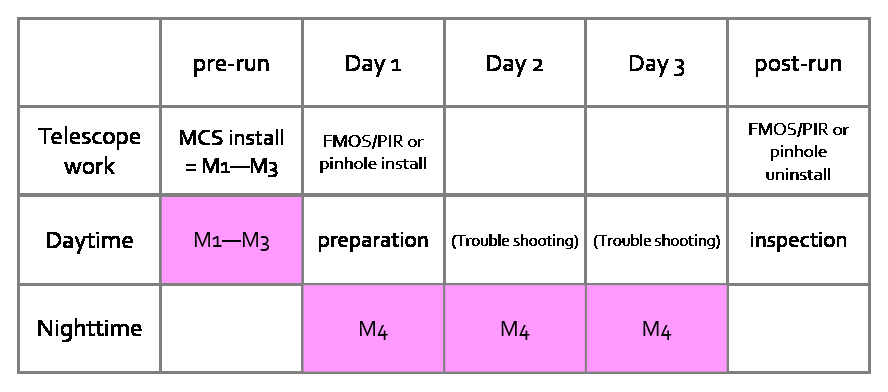
\includegraphics[width=81mm]{timetable_run1.eps}
	\end{center}
	\vspace*{-5mm}
	\caption{Time table of Run 1.}
	\label{fig:run1}
\end{minipage}
\end{tabular}
\end{center}
\end{figure}

%---------------------------------------------------
% Run 2
%---------------------------------------------------
\begin{figure}[!ht]
\begin{center}
\begin{tabular}{c}
\begin{minipage}{0.95\hsize}
\paragraph{Run 2 : 7 days  (Figure \ref{fig:run2})}
	\begin{itemize}
	\item 1 day (daytime) for P-1 -- P-3, P-5 :
	(1) check PFI/Popt2 standing by,
	(2) install POpt2 to the prime focus,
	(3) check PFI functions, and
	(4) measure x/y offset of PFI rotation center on MCS
	\item 0.5 day (daytime) for P-4 :
	(1) verify  MCS performance
	\item 1.5 days (nighttime) for P-6 :
	(1) verification of A\&G camera functions 
	\item 2.5 days (nighttime) for P-7 :
	(1) correct WFC shift/tilt with respect to the primary mirror
	\item 1.5 days (daytime) for P-8 :  
	(1) confirm fixed fiducial fiber positions on F3C (refine the PFI-MCS relation)
	\item 1.5 days (nighttime) for P-9 :
	(1) Telescope Pointing Analysis
	\item 0.7 day (daytime) for F-1 : 
	(1) connect Cable B to PFI and SpS (SM1/2/3)
	\item 1.8 day (daytime) for F-2 :  
	(1) confirm  the fiber identifications (SM1/2/3)
	\item 1.5 days (daytime) for A-1 : 
	(1) calibration of Cobras (SM1/2)
	\item 1.5 days (1.5-day nighttime) for A-2 : 
	(1) PSF measurement through the entire system (SM1/2/3)	
\end{itemize}
\end{minipage} \\
\begin{minipage}{0.8\hsize}
	\begin{center}
	\vspace*{5mm}
	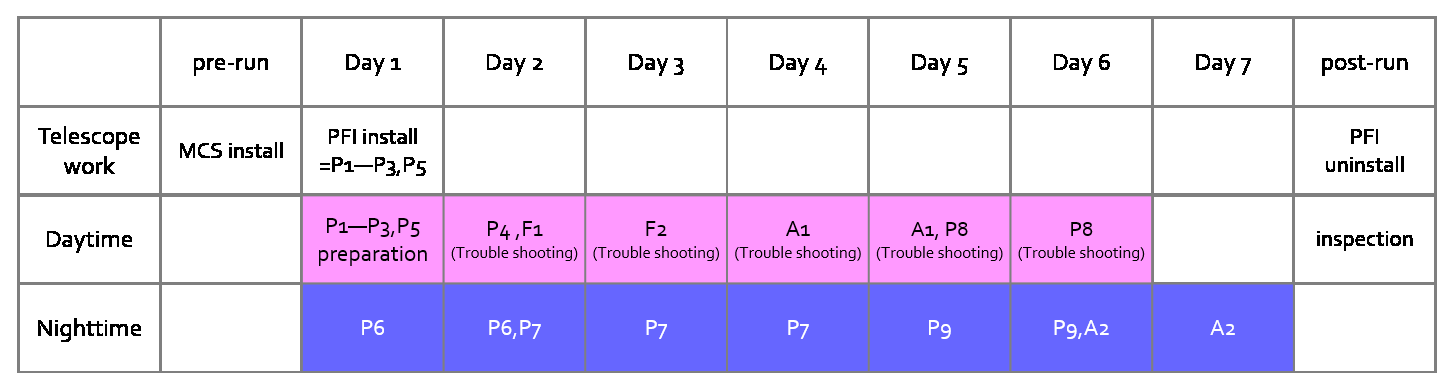
\includegraphics[width=135mm]{timetable_run2.eps}
	\end{center}
	\vspace*{-5mm}
	\caption{Time table of Run 2.}
	\label{fig:run2}
\end{minipage}
\end{tabular}
\end{center}
\end{figure}

%---------------------------------------------------
% Run 3
%---------------------------------------------------
\begin{figure}[!ht]
\begin{center}
\begin{tabular}{c}
\begin{minipage}{0.95\hsize}
\paragraph{Run 3 : 4 days  (Figure \ref{fig:run3})}
	\begin{itemize}
	\item 4 days (nighttime) for P-10 : 
	(1) 1st-pass distortion map
	\item 1.5 days (daytime) for A-1 : 
	(1) calibration of Cobras (SM3/4)
	\item 1.5 days (1.5-day daytime) for A-2 : 
	(1) PSF measurement through the entire system (SM1/2/3)
	\end{itemize}
\end{minipage} \\
\begin{minipage}{0.8\hsize}
	\begin{center}
	\vspace*{5mm}
	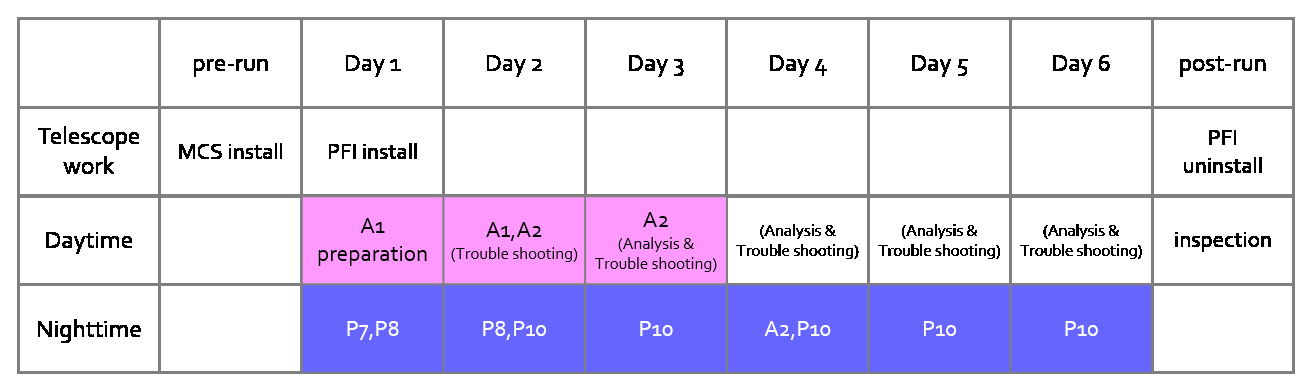
\includegraphics[width=94.5mm]{timetable_run3.eps}
	\end{center}
	\vspace*{-5mm}
	\caption{Time table of Run 3.}
	\label{fig:run3}
\end{minipage}
\end{tabular}
\end{center}
\end{figure}

%---------------------------------------------------
% Run 4
%---------------------------------------------------
\begin{figure}[!ht]
\begin{center}
\begin{tabular}{c}
\begin{minipage}{0.95\hsize}
\paragraph{Run 4 : 6 days  (Figure \ref{fig:run4})}
	\begin{itemize}
	\item 2 days (nighttime) for P-10 : 
	(1) 1st-pass distortion map
	\item 0.4 day (daytime) for F-1 :  
	(1) connecting Cable B to PFI and SpS (SM4)
	\item 0.6 day (daytime) for F-2 :  
	(1) confirmation of  the fiber identifications (SM4)
	\item 1.5 days (1.0-day daytime and 0.5-day nighttime) for A-2: 
	(1) PSF measurement through the entire system (all SMs)
	\item 3.5 days (nighttime) for A-3: 
	(1) 2nd-pass distortion map
	\end{itemize}
\end{minipage} \\
\begin{minipage}{0.8\hsize}
	\begin{center}
	\vspace*{5mm}
	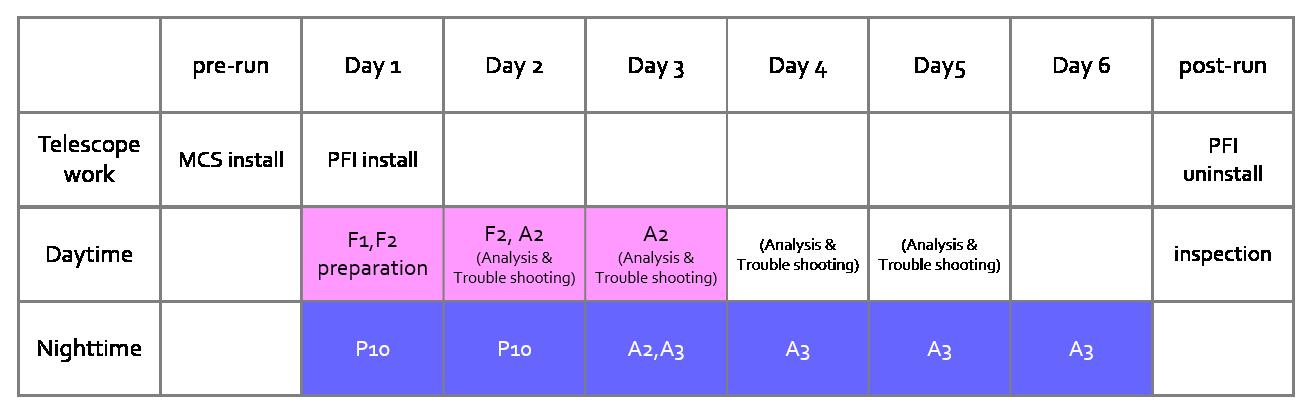
\includegraphics[width=121.5mm]{timetable_run4.eps}
	\end{center}
	\vspace*{-5mm}
	\caption{Time table of Run 4.}
	\label{fig:run4}
\end{minipage}
\end{tabular}
\end{center}
\end{figure}


%---------------------------------------------------
% Run 5
%---------------------------------------------------
\begin{figure}[!ht]
\begin{center}
\begin{tabular}{c}
\begin{minipage}{0.95\hsize}
\paragraph{Run 5 : 6 days  (Figure \ref{fig:run5})}
	\begin{itemize}
	\item 3 days (nighttime) for A-3:
	(1) 2nd-pass distortion map
	\item 3 day (dark-night) for A-4 :
	(1) performance verification I
	\end{itemize}
\end{minipage} \\
\begin{minipage}{0.8\hsize}
	\begin{center}
	\vspace*{5mm}
	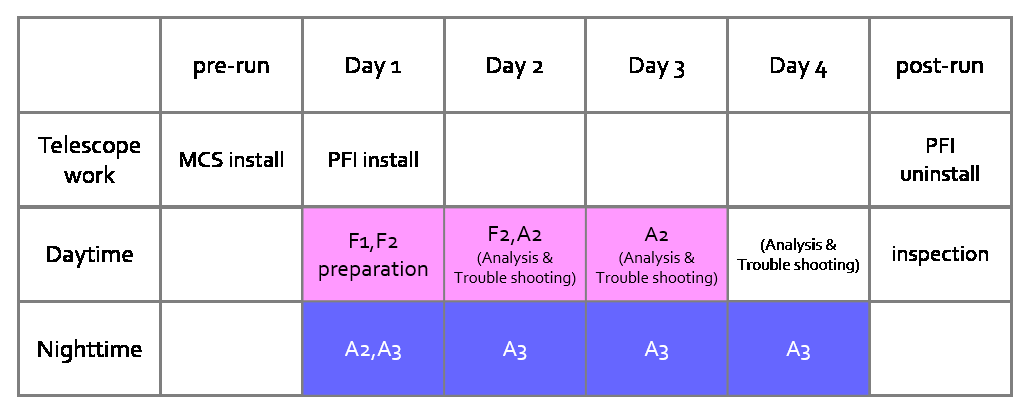
\includegraphics[width=121.5mm]{timetable_run5.eps}
	\end{center}
	\vspace*{-5mm}
	\caption{Time table of Run 5.}
	\label{fig:run5}
\end{minipage}
\end{tabular}
\end{center}
\end{figure}

%---------------------------------------------------
% Run 6
%---------------------------------------------------
\begin{figure}[!ht]
\begin{center}
\begin{tabular}{c}
\begin{minipage}{0.95\hsize}
\paragraph{Run 6 : 4 days  (Figure \ref{fig:run6})}
	\begin{itemize}
	\item 2 days (dark-night) for A-4 : 
	(1) performance verification I
	\item 2 days (dark-night) for A-5 :
	(1) performance verification II (stabilization)
	\end{itemize}
\end{minipage} \\
\begin{minipage}{0.8\hsize}
	\begin{center}
	\vspace*{5mm}
	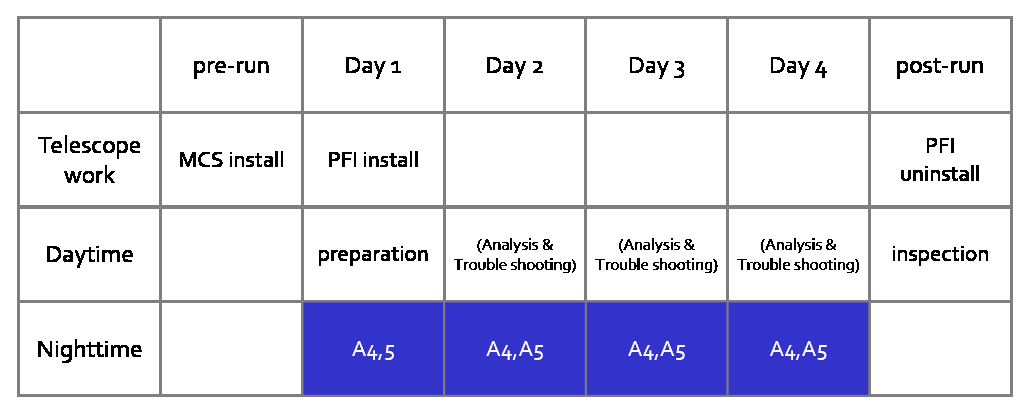
\includegraphics[width=94.5mm]{timetable_run6.eps}
	\end{center}
	\vspace*{-5mm}
	\caption{Time table of Run 6.}
	\label{fig:run6}
\end{minipage}
\end{tabular}
\end{center}
\end{figure}

%---------------------------------------------------
% Run 7 and 8
%---------------------------------------------------
\begin{figure}[!ht]
\begin{center}
\begin{tabular}{c}
\begin{minipage}{0.95\hsize}
\paragraph{Runs 7 and 8 : 4 days  (Figure \ref{fig:run7})}
	\begin{itemize}
	\item 4 days (dark-night) for A-5 :
	(1) performance verification II (stabilization)
	\end{itemize}
\end{minipage} \\
\begin{minipage}{0.8\hsize}
	\begin{center}
	\vspace*{5mm}
	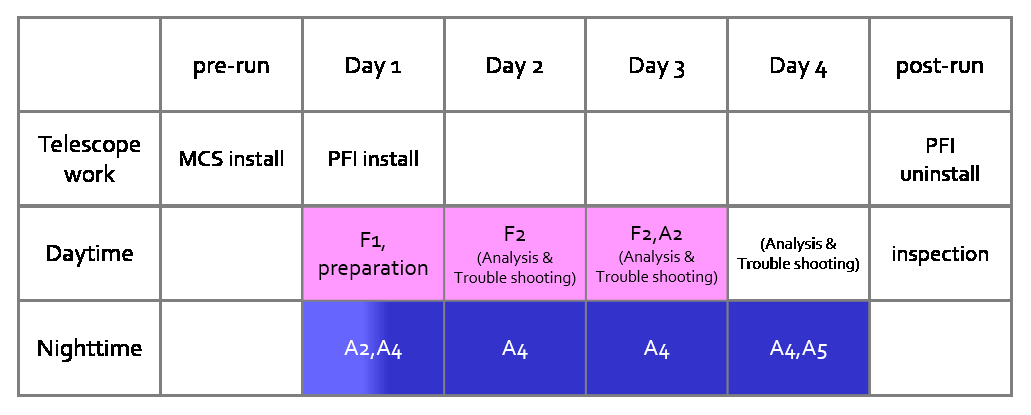
\includegraphics[width=94.5mm]{timetable_run7.eps}
	\end{center}
	\vspace*{-5mm}
	\caption{Time table of Runs 7 and 8.}
	\label{fig:run7}
\end{minipage}
\end{tabular}
\end{center}
\end{figure}


%--------------------------------------------------------------
%  Table: expected runs and nights
%--------------------------------------------------------------
\setlength{\tabcolsep}{1mm}{
\begin{table}[!ht]
\begin{center}
\caption{
Expected days for commissioning.
Note that Year/Month in column 2 are just roughly set assuming the latest schedule of each subsystems and that scientific operation will start in the S20B semester.}
%\scriptsize
\footnotesize
\begin{tabular}{*{3}{c}|*{4}{c}}\label{tbl:CountDates} \\ \hline
Run	 & Year/  &\#days & seq.	& daytime & night-sky  &  dark-sky\\
	& Month	&	&	 & is OK & is needed  &  is needed  \\ \hline \hline
1	& 2017/08		& 3*	& M1--3		& (1*)	& 0		& 0	\\
	& --2019/02	& 		& M4			& 3		& 0		& 0	\\ \hline
2	& 2019/02	& 7 (14**)	& P1--P3,P5	& 1 	& 0 	& 0	\\
	&	&					& P4			& 0.5 	& 0 	& 0	\\
	&	&					& P6  			& 0 	& 1.5 	& 0	\\
	&	&					& P7  			& 0 	& 2.5 	& 0	\\
	&	&					& P8  			& 1.5 	& 0 	& 0	\\
	&	&					& P9  			& 0 	& 1.5 	& 0	\\
	&	&					& F1 (SM1,2)	& 0.7 	& 0 	& 0	\\
	&	&					& F2 (SM1,2)	& 1.8 	& 0 	& 0	\\
	&	&					& A1 (SM1,2)	& 1.5 	& 0 	& 0	\\
	&	&					& A2 (SM1,2)	& 0 	& 1.5 	& 0	\\ \hline
3	& 2019/06	& 4 (7**)	& P11 			& 0 	& 4 	& 0	\\
	&	&					& A1 (SM3,4)	& 1.5 	& 0 	& 0	\\
	&	&					& A2 (SM1,2)	& 1.5 	& 0 	& 0	\\ \hline
4	& 2019/09	& 6 (8**)	& P10			& 0		& 2 	& 0	\\
	&	& 					& F1 (SM3,4)	& 0.4 	& 0 	& 0	\\
	&	&					& F2 (SM3,4)	& 0.6 	& 0 	& 0	\\
	&	&					& A2 (all SMs)	& 1.0 	& 0.5 	& 0	\\
	&	&					& A3			& 0		& 3.5	& 0	\\ \hline
5	& 2019/10	& 6			& A3			& 0		& 3		& 0	\\
	&	&					& A4			& 0		& 0 	& 3	\\ \hline
6	& 2019/12	& 4			& A4			& 0		& 0 	& 2\\
	&	&					& A5			& 0		& 0 	& 2	\\ \hline
7	& 2020/04	& 4			& A5			& 0		& 0 	& 4	\\ \hline
8	& 2020/07	& 4			& A5			& 0		& 0 	& 4	\\ \hline \hline
\multicolumn{2}{r}{in total}& 38 (50**) \\ \hline
\end{tabular}
\\
* telescope can be used for other instruments \\
** day-time and night-time works are counted independently
\end{center}
\end{table}

\clearpage

\subsection{Relationship among Individual Sequence}
Some sequences can be carried out in parallel, but some should in series.
Table \ref{tbl:Rel_Seq} shows the relationship among the individual sequences.
The rows are commissioning sequences related to each sequence in the columns.
``X" means required sequences.
For example, prior to the sequence M--3, M--2 (and hence M--1) should be succeeded.

%--------------------------------------------------------------
%  Table: the relation ship of commissioning sequence 
%  A sequence (top) marked with X is need prior to other sequence (row)
%--------------------------------------------------------------
\begin{table}[!ht]
\caption{
The relation of commissioning sequences.}
\label{tbl:Rel_Seq}
\begin{center}
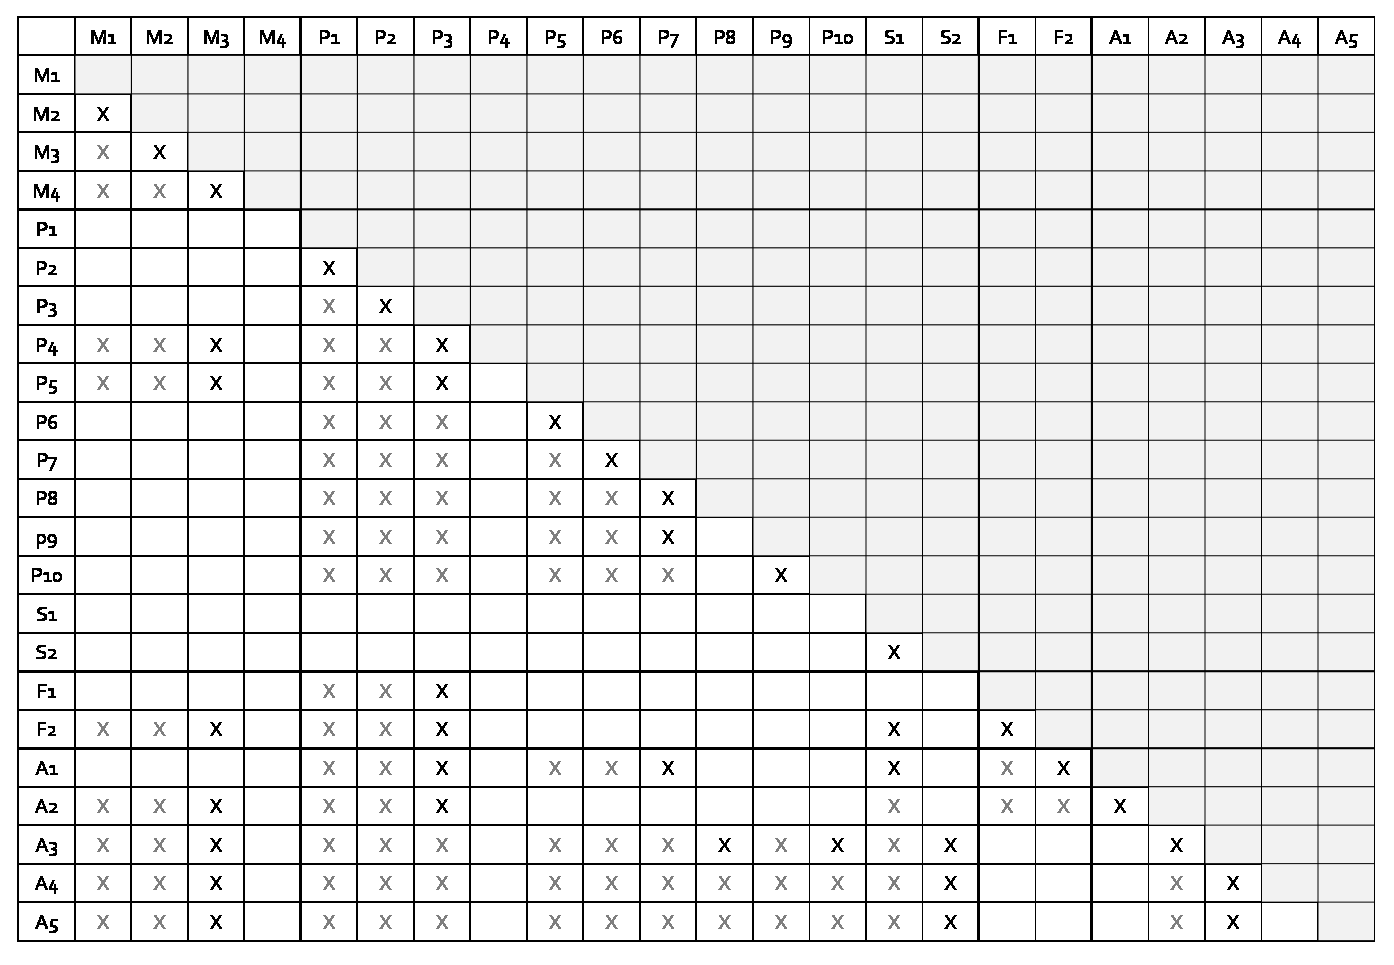
\includegraphics[width=170mm]{relationship_sequences.eps}
\end{center}
\end{table}


